%  LaTeX support: latex@mdpi.com
%  MDPI MAKE submission — main_paper_MAKE48.tex
%  Version 48: response to the editorial language/reference check on MAKE47
%    - [lang] removed the flagged phrase "actually occur(red)" (3 sites:
%      Sec. 2, Sec. 3.2.2, Sec. 5.7 intro) and reduced other uses of
%      "actually"; "multi-seed" is standard ML terminology (the flagged
%      "multi-see" is a substring artifact) and is kept unchanged
%    - [refs] bibliographic completion/correction of the entries flagged
%      "requiring validation": rifai2011cae (28th ICML, pp. 833-840, not
%      "Vol. 28"), ghahramani2005infinite -> author order Griffiths;
%      Ghahramani + pp. 475-482, nazari2023geometric (+2023, pp.
%      25834-25857), kato2020rdae (+2020, pp. 5166-5176), kingma2014vae /
%      higgins2017betavae (+venue location and dates), netzer2011reading /
%      hoffman2016elbo (+workshop location), krizhevsky2009learning
%      (publisher address)
%    - [refs] DOIs added to journal-article entries (bengio2013, fefferman
%      2016, facco2017, ceruti2014, camastra2016, allegra2020,
%      tippingbishop1999, johnsson2015, lecun1998)
%    - no reference added or removed: numbering [1]-[37] unchanged
%  ---- Version 47 changes below ----
%  Version 47: final pre-submission polish per MAKE46_投稿前最終確認事項.md
%    - [1] Figure fig:en caption: "failure mode ... detected by the AU
%      signal" -> observation ("no substantial truncation observed") +
%      diagnostic interpretation ("consistent with insufficient beta")
%    - [2] confirmed: no "a generous m is safe" phrasing remains in body
%    - [3] Sec. 5.2: "surrogate prediction ... is confirmed on ground
%      truth" -> "consistent with the surrogate expectation" under this
%      synthetic setting
%    - [4] Table tab:applicability: synthetic row -> "Validated on the
%      tested synthetic manifolds when MSE-triggered margin enlargement is
%      allowed"; Conv-VAE row -> "when sufficient truncation can be induced
%      under the chosen architecture and training schedule"
%    - [5] cross-references, citation order, and Appendix A.1 distinctions
%      re-verified after recompile
%  ---- Version 46 changes below ----
%  Version 46: revisions in response to review45.md + MDPI compliance
%    - [review45 1.1] Appendix A.1 (i): exactness split by coordinate type
%      (already in place from v45; wording confirmed); Remark note aligned
%    - [review45 1.2] d*_eff(beta) defined as an interpretive quantity for
%      the nonlinear experiment, not directly estimated from it
%    - [review45 1.3] "clear AU = m pattern" -> "near-diagonal AU-m
%      relationship"
%    - [review45 3.2] Sec. 4.2 title -> "Surplus-Dimension Truncation in a
%      Water-Filling Surrogate"
%    - [review45 3.3] Remark (i): "a generous m is safe for VAEs" ->
%      conservative strategy phrasing; Sec. 2 "safety device" -> "mechanism"
%    - [review45 4.2] beta strengthening: "necessary condition" -> "may be
%      required before AU-based verification can be informative"
%    - [review45 4.4] TwoNN global-metric sentence made more careful
%    - [review45 6.3] Sec. 1.2 "predicts" -> "motivates the expectation"
%    - [MDPI] \reftitle{References} added (missing section heading)
%    - [MDPI] abstract compressed to ~200 words (was ~306), includes
%      review45 2.2 "Under the tested settings" scoping
%    - [MDPI] \institutionalreview{Not applicable.} and
%      \informedconsent{Not applicable.} added
%    - [MDPI] \supplementary{} added (anonymized review archive; public
%      GitHub + Zenodo DOI upon acceptance)
%    - [MDPI] \acknowledgments{} added with generative-AI use disclosure
%      (code generation assistance, English checking, proofreading)
%    - [MDPI] \funding reworded to "This research was funded by ..."
%    - [refs] five related lab publications added and cited:
%      obata2025manifold (NOLTA2025 preliminary study; Sec. 1.2),
%      okamoto2023latent, jinno2023multimodal, dai2024latent (Sec. 2),
%      dai2026island (Sec. 2); citation order verified (37 cited = 37 items)
%  ---- Version 45 changes below ----
%  Version 45: revisions in response to review44.md
%    - [R1] Appendix A.1 (and Remark): approximation exact on truncated
%      coordinates only; on active coordinates the aggregated-posterior
%      mismatch is assumed negligible (PPCA variance matching motivates,
%      does not establish, exact vanishing)
%    - [R2] Sec. 5.6.1: AU = m pattern "flags the diagnostic condition
%      'no substantial truncation observed'", consistent with beta too
%      small (no direct causal detection); Table tab:failure first row
%      likewise
%    - [R3] abstract: "standard beta" -> tested Conv-VAE schedule with
%      beta_max = 4, no truncation observed within tested range;
%      conclusions likewise
%    - [R4] abstract: natural-image inflation concretized (latent TwoNN
%      increased when reference bottleneck exceeded the provisional
%      consistency region)
%    - [R5] Sec. 1.2: conservative strategy "may be useful when KL-induced
%      truncation is effective", a hypothesis checked by Step 3
%    - [R6] Sec. 4.3: "sketch of sufficient conditions" -> "heuristic
%      description of conditions that may support conditional stability"
%    - [R7] Sec. 5.3.1: operational primary reference \hat d_ID = 10
%      (rounded TwoNN); MLE 11.3-11.9 as order-of-magnitude cross-check
%    - [R8] Table tab:mnist_s1 caption: Table tab:mnist_s3 is the
%      candidate-VAE latent cross-check (diagnostic only)
%    - [R9] Sec. 5.6.2: d* >> m stated under the surrogate interpretation
%    - [R10] Table tab:applicability: synthetic row "validated ... when
%      adaptive margin enlargement is allowed"; Conv-VAE row "conditional
%      applicability after architecture- and schedule-dependent truncation
%      is induced"
%    - [R11] "verifying post training" -> "verifying after training"
%    - [R12] "on the specific MNIST grid used here" -> "for the specific
%      MNIST grid and evaluation protocol used here"
%    - [R13] V1/V2 pass: "same order" -> AU lies within the operational
%      range defined relative to the Step-1 reference
%  ---- Version 44 changes below ----
%  Version 44: revisions in response to review43.md
%    - [R1] Appendix A.1: D_j(R_j) redefined as the residual variance
%      contribution (not "distortion reduction"); R_j in nats; L_j stated
%      as maximized up to additive constants; lambda_j / tau^2 defined
%    - [R11] aggregated-posterior mismatch on active coordinates stated as
%      "assumed negligible" at the specific linear-Gaussian optimum
%    - [R12] "underestimating truncation" reworded: surrogate tends to
%      predict weaker truncation / may overestimate active dimensions
%    - [R2] d*(beta) > 512 restated as observation + surrogate-consistent
%      interpretation (d*_eff(beta) > 512); Sec. 1.2 contribution likewise
%    - [R3] "clear induced saturation" -> reduction in activation ratio /
%      stronger truncation within tested range; no stable-plateau claim
%    - [R4] Figure fig:en regenerated (EN_conv_vae_extended_m_v44) with
%      "Step-1 ref. \hat d_ID = 10" label; caption notes the reference-AE
%      origin of the value (Figs. 2/3 already render \hat d_ID)
%    - [R5] "safe-side operation" -> conservative operating strategy
%    - [R6][R7] abstract: seed design made explicit (3-5 synthetic /
%      3 real); "three steps ... reproducible decision rule" limited to
%      the pre-specified Step-3 rule + complementary MSE diagnostics
%    - [R8] Sec. 5.3.3: AE window [10,24] derivation made reproducible
%      (round(TwoNN)=10; ceil(2*MLE)=24), flagged as MNIST-specific
%    - [R9] Sec. 4.1: \hat d_ID as practical reference point, not a formal
%      lower bound for real data
%    - [R13][R14] Torus: "self-intersecting (an immersion)" weakened to
%      consistency statement; "deterministic" -> identical across the five
%      tested seeds
%    - [R15] Table tab:applicability: "Fully applicable" -> ground-truth
%      validated with an adaptive margin diagnostic
%    - [R16] Table tab:failure: "Likely cause" -> "Diagnostic
%      interpretation"; lower-V2 row reworded as consistency statement
%    - [R17] m_ref ~ 2 \hat d_ID on natural images labeled a provisional
%      consistency region, not a validated selection rule
%    - [R18] Allegra et al.: "model exactly" -> "provide a related
%      treatment of"
%    - [R19] Table tab:notation: d_emb entry now relates to ideal manifold
%      dimension d (not d_ID)
%    - [R20] Fig. 2 caption: single-seed sweep for visualization; principal
%      verification decisions from 3-seed Table tab:mnist_s3 / Fig. 3
%    - [R21] "organized into three contributions" fixed
%    - [R22] Sec. 4 title -> "Theoretical Motivation and Interpretive
%      Surrogates"
%    - [R23] DANCo claim conditioned; [R24] "the manifold dimension" in the
%      Introduction replaced by an estimate of local intrinsic
%      dimensionality
%    - [R25] Sec. 5.1: +/- values are inter-seed standard deviations
%    - [R26] "identical"/"unanimous" -> explicit per-seed statements
%  ---- Version 43 changes below ----
%  Version 43: revisions in response to
%  MAKE投稿論文_修正指摘と改善案.md (pre-submission review)
%    - [T1] title changed from "Choosing ... from the Intrinsic Dimension"
%      to "Intrinsic-Dimension-Guided Bottleneck Selection ... with
%      Active-Unit Diagnostics" (protocol/diagnostics framing)
%    - [T2] abstract rewritten: conditional diagnostic protocol; VAE rule
%      m >= 2*dID stated as generous-candidate + post-training check, not a
%      guarantee; "grid-best" -> "best observed"; AU explicitly not a
%      general estimator of intrinsic/embedding dimension
%    - [T4] Prop. 1 restricted to idealized zero-error continuous
%      reconstruction; d_emb >= d_ID framed as geometric motivation, not an
%      empirically verifiable inequality involving \hat d_ID; Prop. 2
%      explicitly not a coordinate-wise activation theorem for nonlinear
%      VAEs; ELBO-surgery exactness limited to the specific global optimum;
%      Prop. 3 demoted to a heuristic conditional-stability rationale
%      (no Proposition environment; all cross-references updated)
%    - [T5] AUsat notation-table entry reworded; AU coordinate dependence
%      (non-invariance under latent rotations/reparameterizations) added
%    - [T6] Step-1 reference AE vs Step-3 candidate VAE separation made
%      explicit; single-seed m_ref sweep vs 3-seed verification clarified;
%      subsampling-CI scope limited; "stable" claims conditioned on the
%      tested datasets/architectures/estimators
%    - [T7] V1/V2 restated as operational screening criteria; explicit
%      list of what a pass does NOT imply
%    - [T8] training-run accounting table added (Table tab:cost);
%      VAE 0.9-point gap quantified, no equivalence claim; AE single-seed
%      probe results flagged as descriptive
%    - [T9] fixed-beta surrogate vs cyclical KL annealing distinguished
%      (beta_max = schedule parameter); annealing schedule specified;
%      natural-image mechanisms framed as untested hypotheses with an
%      operational definition of manifold entanglement; SVHN raw-input
%      TwoNN not treated as ground truth; tau_eff^2 flagged post hoc
%    - [T10] fixed-order subset rationale and caveat added
%    - [T11] related work extended: ID-estimator limitations
%      (Camastra & Staiano 2016; Allegra et al. 2020) and AU definition
%      limits
%    - [T12] Table tab:ea simplified (notes moved to caption); Figure
%      fig:e4_dualaxis split into 4 panels (E4_mnist_dualaxis_v43);
%      Figure fig:e4_multiseed labels reworded (E4_300ep_multiseed_v43);
%      Figure fig:ep caption no longer suggests isometry is irrelevant
%    - [T13] Sec. 1.2 contributions reorganized (methodological /
%      diagnostic / empirical / theoretical motivation); Sec. 1.4 trimmed
%  ---- Version 42 changes (in response to Peer_Review_Report41.md) below ----
%    - [Major 2] Fashion-MNIST Step 3 upgraded to a 3-seed verification
%      (Exp-Fashion-MS, 300 ep)
%    - [Major 2] Exp-ConvV-HiBeta upgraded to a 3-seed verification
%      (Exp-ConvV-HiBeta-MS)
%    - [Major 1] hypotheses on why latent-geometry distortion is so
%      pronounced on natural images (manifold entanglement, need for
%      hierarchical latents) added to Secs. 5.6.2 and 6.4
%    - [Major 3] discussion of the aggregated-posterior mismatch
%      KL(q(z)||p(z)) during nonlinear optimization added to Remark 2 and
%      Appendix A.1 (ELBO surgery reference added)
%    - [Minor 1] abstract: specific numbers trimmed, emphasis shifted to
%      the closed-loop protocol
%    - [Minor 2] Figures 2 (E4_300ep_multiseed) and 5 (Exp_ConvV_HiBeta)
%      regenerated with B/W-print-safe line styles and larger fonts
%    - [Minor 3] Step 2: the multiplier 2 re-emphasized as a buffer for the
%      unknown d_emb
%  ---- Version 41 changes (in response to Review_codex40.txt) below ----
%    - DANCo wording in Sec. 2 fixed: not a primary estimator, used as an
%      auxiliary robustness cross-check on MNIST latents (Minor 1)
%    - full audit of references (all cited, citation-order numbering) and
%      of figure/table in-text mentions
%  ---- Version 40 changes (in response to Review_codex39.txt) below ----
%    - Sec. 4 real-data-validation question rephrased: "does the full
%      protocol work on MNIST, what evidence is available for
%      Fashion-MNIST" (Minor 1)
%    - repository URL/DOI (Minor 2) and MDPI production placeholders
%      (presentation 1) left for the submission/editorial stage
%  ---- Version 39 changes (in response to Review_codex38.txt) below ----
%    - contradictory Fashion-MNIST sentence in Sec. 4.3.6 rewritten:
%      Step 1 is multi-seed, VAE-side AU verification is a single-seed
%      preliminary observation (Minor 1)
%    - Sec. 4.1 multi-seed sentence refined to "used for the principal
%      verdicts"; in-text exploratory single-seed summaries acknowledged
%      (Minor 2)
%    - Sec. 4.3.3 parenthetical added: AE window = TwoNN--MLE envelope,
%      VAE m_ver = primary TwoNN rule (Minor 3)
%    - Sec. 1.2 contribution claim made exact: multi-seed AU verification
%      on MNIST; Step-1 stability via subsampling CIs, estimator
%      cross-checks, and the 3-seed reference-model comparison (Minor 4)
%    - V2 threshold-invariance note: displayed range rounded conservatively
%      (mean lower edge 2.24) (presentation 2)
%    - natural-image table caption: Pope et al. agreement limited to
%      CIFAR-10 (presentation 3)
%    - abstract boundary-case detail lightly trimmed (presentation 4)
%    - MDPI production placeholders (dates, article no., DOI) left
%      for the editorial stage (presentation 1); author ORCID iDs filled in
%  Compiled with official mdpi.cls
%  Compile: pdflatex main_paper_MAKE42.tex  (x3 for cross-references)

%=================================================================
\documentclass[make,article,submit,pdftex,moreauthors]{Definitions/mdpi}

%=================================================================
% MDPI internal commands — do not modify
\firstpage{1}
\makeatletter
\setcounter{page}{\@firstpage}
\makeatother
\pubvolume{8}
\issuenum{1}
\articlenumber{0}
\pubyear{2026}
\copyrightyear{2026}
%\externaleditor{Firstname Lastname}
\datereceived{ }
\daterevised{ }
\dateaccepted{ }
\datepublished{ }

%=================================================================
% Notation shorthands (kept in sync with main_paper_NN35.tex)
\newcommand{\dID}{d_{\mathrm{ID}}}
\newcommand{\hatdID}{\hat{d}_{\mathrm{ID}}}
\newcommand{\dz}{m}
\newcommand{\dtrue}{d_{\mathrm{true}}}
\newcommand{\Jg}{J_g}
\newcommand{\R}{\mathbb{R}}
\newcommand{\kap}{\kappa}
\newcommand{\AUsat}{\mathrm{AU}_{\mathrm{sat}}}
\newcommand{\demb}{d_{\mathrm{emb}}}
\newcommand{\mknee}{m^{\mathrm{knee}}}
\newcommand{\dstar}{d^{*}(\beta)}

%=================================================================
\Title{Which Signals Actually Support the Choice of a VAE Latent
Dimension? A Pre-Registered Comparison of Intrinsic-Dimension,
Activity-Based and Pruning Criteria}

% ORCID IDs
\newcommand{\orcidauthorA}{0009-0001-1209-0918} % Chika Obata
\newcommand{\orcidauthorB}{0000-0002-4070-4585} % Mizuki Dai
\newcommand{\orcidauthorC}{0000-0002-0431-5769} % Kenya Jin'no

\Author{Chika Obata $^{1}$\orcidA{},
        Mizuki Dai $^{1}$\orcidB{}, and
        Kenya Jin'no $^{1,}$*\orcidC{}}

\AuthorNames{Chika Obata, Mizuki Dai, and Kenya Jin'no}

\address{%
$^{1}$ \quad Department of Intelligent Systems,
  Faculty of Information Engineering,
  Tokyo City University,
  1-28-1 Tamazutsumi, Setagaya-ku, Tokyo 158-8557, Japan;
  g2332016@tcu.ac.jp (C.O.); g2591402@tcu.ac.jp (M.D.)}

\corres{Correspondence: kjinno@tcu.ac.jp; Tel.: +81-3-5707-0104 (K.J.)}

%=================================================================
\abstract{%
Choosing the latent dimension of a variational autoencoder is usually
done by grid search. Cheaper criteria have been proposed, based on an
intrinsic-dimension estimate of the data or on how many latent variables
stay active after training. Under one protocol fixed in advance, we asked
which of these signals actually supports the decision. We compared
intrinsic-dimension guidance, two published selection algorithms, a
pruning method with a reconstruction constraint, an automatic-relevance
variant, grid search, coarse search and fixed dimensions, across four
datasets, five seeds and five regularisation settings. Guidance by
intrinsic dimension gave no measurable advantage: a plain ascending scan
under the same quality criterion matched or beat it at lower cost on every
dataset, and the guidance step declined to apply on two of three image
datasets. The activity readout carried no information beyond a matched set
of random features. Nearly every criterion was governed by a free
threshold, and the dimension selected moves several-fold when that
threshold varies; the ordering of methods by this sensitivity is itself
reproducible, and one method is insensitive to it. We report these
negative results, the sensitivity ordering, and the implementation failure
modes we met, as the contribution.}

\keyword{variational autoencoder; latent dimension; intrinsic dimension;
active units; model selection; pruning; automatic relevance determination;
reproducibility; negative results; pre-registration}

%=================================================================
\begin{document}

% ============================================================
% 改訂稿 NN49 / MAKE49 骨格
% 枠組み: 「ID 誘導による高速な次元選択法の提案」から
%         「VAE の次元選択における診断と落とし穴の実証研究」へ
% 根拠: MAKE49_段階1〜8 の各報告書
% ============================================================

\section{Introduction}\label{sec:intro}

The latent dimension of a variational autoencoder has to be set before
training, and it is usually set by grid search: train a model at each
candidate capacity and keep the one that performs best. This is reliable
and expensive, and a number of cheaper criteria have been proposed in its
place. Some estimate the intrinsic dimension of the data and use it to
place a search window. Others train a single large model briefly and read
off how many latent coordinates remain in use, either from the variance of
the posterior means or from a classification of the latent variables into
types. Others again prune during training, under an explicit constraint on
reconstruction quality or under a prior that suppresses irrelevant axes.

Each of these criteria has been reported to work on the datasets its
authors used. What has not been established is how they behave against one
another under a single protocol: with the same quality target, the same
accounting of cost, the same number of seeds, and the same treatment of
the cases where a method declines to answer. Without that, it is difficult
to know whether a reported saving reflects the criterion or the conditions
in which it was measured.

This paper reports such a comparison. We fixed the protocol in advance ---
the quality target, the budget, the termination states, the decision rules
and the number of seeds --- and recorded every subsequent change with its
reason. We then ran intrinsic-dimension guidance, two published selection
algorithms, a constrained pruning method, an automatic-relevance variant,
grid search, coarse search and fixed dimensions across four datasets, five
seeds and five settings of the regularisation weight.

Our results are largely negative, and we report them as the contribution.
Guidance by an intrinsic-dimension estimate bought nothing that a plain
ascending search under the same quality target did not, and it declined to
apply on the datasets it was not developed on. The activity-based readout
was no more stable than the readout it was meant to improve on, and in a
prediction task fixed in advance it was not distinguishable from random
features of the same number. The one criterion that transferred well is
not ours: it coincides with a constraint already used by an existing
pruning method, and we say so.

What does emerge is a measurement. Nearly every rule we examined is
governed by a free parameter, and the dimension it selects moves
severalfold when that parameter is varied. The methods differ in this
sensitivity by two orders of magnitude, the ordering reproduces across
datasets, and one method sits at zero. We also document three
implementation defects of a single kind --- a sum written as a mean --- that
left training intact and the resulting curves plausible. Section~\ref{sec:results}
presents the measurements and Section~\ref{sec:discussion} discusses what
would change the conclusion.

\section{Related Work}\label{sec:related}

Two overlaps with existing work bear on how this paper should be read, and
we state them before the survey rather than after it.

First, the appendix of the intrinsic-dimension selection algorithm that we
use as a comparison method already proposes choosing the latent dimension
from the variable types of a briefly trained model. That is the same idea
as the activity-based verification this line of work set out to study. Its
authors describe it and set it aside, reporting that variable types are
unreliable early in training. Our measurements reproduce that instability,
and extend the comparison to long training, where we find that the
advantage they were weighing does not appear in either direction.

Second, the pruning method we added during revision selects the smallest
capacity that satisfies an explicit upper bound on reconstruction error.
The quality criterion used throughout this paper is that construction. We
do not present it as a contribution, and in Section~\ref{sec:res_threshold}
we report the correspondence quantitatively.

\subsection{Dimensionality Reduction and Intrinsic Dimension}\label{sec:rel_dr}

Reducing dimension by finding coordinates that preserve structure is an old
problem. Principal component analysis gives a linear answer; Isomap and
locally linear embedding give nonlinear ones by preserving geodesic or
neighbourhood structure. These methods produce an embedding, not a
criterion for how many coordinates a separately trained generative model
should have, which is the question here.

Estimating the intrinsic dimension of a sample is a related but distinct
task. We use the two-nearest-neighbour estimator as the primary estimator
and a maximum-likelihood estimator as a cross-check; other families exist,
including concentration-based estimators and graph-based estimators built
from minimal spanning trees or geodesic entropic graphs. We did not
implement a graph-based estimator: the measurements in
Section~\ref{sec:res_id} show that the disagreement we care about is
already visible between the two estimators we do use, and adding a third
would not resolve it. Deep representations have been reported to have
lower intrinsic dimension than their inputs, which is part of the
motivation for reading a latent dimension off such an estimate.

\subsection{Choosing the Latent Dimension}\label{sec:rel_select}

Two published algorithms select the dimension from an intrinsic-dimension
estimate of the representations. The first compares the estimated
dimension of the sampled and the mean representation of a briefly trained
model and returns the largest capacity at which they have not yet
diverged. The second, given in the appendix of the same work, starts from
twice the data estimate, doubles capacity until latent variables of the
unused type appear, and returns the count of the remaining ones. As noted
above, the second is the construction this line of work set out to study
independently.

\subsection{Pruning During Training}\label{sec:rel_prune}

A different strategy trains one large model and removes capacity while
training. One approach places a binary gate on each latent coordinate,
penalises the number of open gates, and holds reconstruction error below a
stated bound by a Lagrange multiplier updated from the constraint
violation; the number of gates left open is the answer. Because the bound
is stated in data space rather than in the latent space, its authors argue
it is easier to set than a regularisation weight --- an argument our
measurements support, and which is why we adopt the same construction as
our common quality target. Another approach replaces the fixed prior with
a hierarchical one whose per-axis variance is fitted to the encoded data,
and reads relevance from that variance; it introduces no threshold of the
kind the other methods rely on, and Section~\ref{sec:res_threshold} shows
what that buys.

\subsection{Active Units and Posterior Collapse}\label{sec:rel_au}

Counting the latent coordinates whose posterior means retain variance is a
standard diagnostic for posterior collapse, and the classification of
latent variables into active, mixed and passive types is a refinement of
it. Both are read from a trained model rather than used to choose its
capacity; the step from diagnostic to selection criterion is the one this
paper evaluates.

\subsection{Relation to Our Earlier Conference Paper}\label{sec:rel_nolta}

A conference paper by the same authors reported that the intrinsic
dimension of the data is informative for bottleneck design and that latent
estimates fall below input estimates, using fully connected models on a
single dataset. It did not consider active units, did not compare against
other selection methods, and did not vary the regularisation weight. The
present paper shares the starting observation and differs in what it
concludes: the comparison it adds does not support using that observation
to place a search window.

% TODO(text): NOLTA2025 との 3 列差分表（会議版 / MAKE47 既存 / 本改訂）を挿入

\section{Evaluation Framework}\label{sec:framework}

Every method is evaluated under the same target, the same accounting and
the same set of outcomes. This section states them; the settings
themselves were fixed before any of the experiments reported here were
run, and each later change is listed with its date and reason in the
supplementary material.

\subsection{Quality Target}\label{sec:framework_quality}

A candidate is acceptable if its validation reconstruction error does not
exceed that of a pre-declared reference model by more than a stated
tolerance. The reference is the largest capacity on the candidate grid,
trained with the same model family, likelihood and regularisation weight
as the candidates, and its cost is charged. The tolerance is the larger of
a relative margin, three times the seed-to-seed standard deviation at the
reference, and an absolute floor that keeps the criterion meaningful when
the reference error is near zero. The resulting target is fixed before any
intervention and is not recomputed afterwards.

As noted in Section~\ref{sec:related}, this is the same construction as
the reconstruction constraint of an existing pruning method, and we make
no novelty claim for it. We state it explicitly because it is the common
yardstick that makes the comparison possible: without a shared target,
methods that optimise different objectives cannot be said to reach the
same quality.

\subsection{Cost Accounting}\label{sec:framework_cost}

Every method is charged up to the point where a model is selected and
trained ready for final evaluation. That includes reference-model
training, intrinsic-dimension estimation, candidate training, the
reference model required by the quality target, any re-search, probe
fitting where a method uses labels, and evaluation. Methods whose search
phase is deliberately short keep that advantage, because the final
training at the selected dimension is charged to every method alike.
Repeated requests for the same configuration within one run of one method
are charged once.

\subsection{Outcomes}\label{sec:framework_outcomes}

A run ends in one of five states: it selected a capacity smaller than the
reference; it found nothing smaller than the reference that met the
target; its estimation step failed a reliability check and it fell back to
a pre-declared conventional search; it exhausted its budget; or it
returned a capacity that cannot be trained. Runs that exhaust the budget
or return a degenerate capacity are reported in the breakdown and are not
removed from the averages. We state this because a comparison that drops
them silently will favour whichever method fails least gracefully.

\section{Theoretical Background}\label{sec:theory}

Two known results motivate the quantities we measure. Neither is a
contribution of this paper and neither is used as a guarantee.

A continuous, self-intersection-free reconstruction of data supported on a
$d$-dimensional manifold requires a latent space at least as large as the
manifold's embedding dimension, which is bounded above by $2d$ for smooth
manifolds. This gives a geometric reason to look near twice an estimate of
the intrinsic dimension when placing a search window. It does not tell us
that an estimate obtained from a particular representation corresponds to
the manifold dimension, nor does it place a lower bound on the average
reconstruction error of a finite sample at a given tolerance. We therefore
treat the factor of two as a default under test and measure its
sensitivity rather than deriving it.

In a linear-Gaussian surrogate with fixed observation noise, the latent
coordinates that remain informative are those whose signal exceeds a
threshold set by the regularisation weight. This gives a reason to expect
that the count of active coordinates responds to that weight. It does not
license reading the count as an estimate of a geometric dimension, and it
does not transfer to the nonlinear models we train. Claims in the earlier
version of this work that went beyond this --- a Jacobian-rank argument, an
unproved upper bound, an effective-noise quantity defined in terms of the
behaviour it was meant to explain, an identification of the activity count
with the variable-type classification, and an inference of direction from
the sign of a divergence term --- have been removed.

\section{Experimental Setup}\label{sec:setup}

\subsection{Objective and Likelihood}\label{sec:setup_loss}

The reconstruction term is summed over input dimensions and averaged over
the batch; the divergence term is summed over latent dimensions and
averaged over the batch. This matters: an earlier version of this work
averaged the divergence over latent dimensions as well, which made the
effective regularisation weight inversely proportional to the very
capacity being varied. Every variational experiment in that version was
affected, and all of them have been re-run. A regression test now checks
that the divergence scales with capacity for fixed per-coordinate
statistics.

The likelihood follows the data type: Bernoulli for the binary image
dataset, Gaussian elsewhere. This is stated in every table and figure,
loss values are never ranked across datasets with different likelihoods,
and the same weight under different likelihoods is not described as the
same strength. The per-pixel mean squared error used for the quality
target is common to all of them.

\subsection{Data, Splits and Repetition}\label{sec:setup_data}

Official training data is split into training and validation portions by a
fixed random draw whose indices are stored; the official test split is
used once, on the checkpoint that validation selected. Subsets are drawn
at random rather than taken from the head of the file. Transformations are
fitted on the training portion only. The main comparison uses five
independent seeds, and the whole procedure --- reference models,
estimation, selection, final training --- is repeated for each; evaluating
one checkpoint five times is not five seeds.

\subsection{Models, Grids and Comparison Methods}\label{sec:setup_methods}

Fully connected encoders and decoders are used for the two
grayscale digit-style datasets and convolutional ones for the other two,
with a candidate grid of twelve capacities for the first three datasets
and ten for the largest. Table~\ref{tab:methods_def} defines the
comparison methods.

\begin{table}[H]
\caption{Comparison methods. Every method is charged for a final training
at the capacity it selects, so that a short search phase is reflected in
the cost rather than removed from it.}
\label{tab:methods_def}
\begin{tabularx}{\textwidth}{lX}
\toprule
\textbf{Method} & \textbf{Selection rule} \\
\midrule
Grid search & Train every capacity on the grid; keep the best validation
reconstruction. Variants use the evidence lower bound or a linear probe. \\
Coarse search & Four log-spaced capacities from the same grid. \\
Fixed dimension & A single capacity fixed before the experiments. \\
FONDUE & Exponential-then-binary search for the largest capacity at which
the estimated dimensions of the sampled and the mean representation differ
by no more than a fifth of the data estimate; threshold computed once and
held. Epoch budget per dataset follows the source, determined for the
datasets it does not cover by the procedure the source describes. \\
FONDUE-VAR & Double capacity from twice the data estimate until unused
variable types appear; return the count of the remaining ones. Run with
both declared settings. \\
GECO + $L_0$ & Gated latent coordinates, penalised by the expected number
of open gates, under a reconstruction bound enforced by a Lagrange
multiplier. \emph{Deviation:} the source uses an augment-reinforce-merge
gradient estimator; we use the hard-concrete relaxation of the same
$L_0$ objective. \\
ARD-VAE & Hierarchical prior with per-axis variance fitted to the encoded
data; relevant axes are those accounting for 99\% of a
sensitivity-weighted variance score. \emph{Deviation:} the source uses the
marginalised Student's~$t$ target; we use a Gaussian with the same
conjugate variance estimate. \\
ID-guided + target & Reference models, estimation, reliability checks,
then every capacity in the window at or below twice the estimate, with a
declared expansion rule; returns the smallest evaluated capacity meeting
the quality target. \\
Ascending scan + target & The same objective without estimation or
reference models: scan the grid upwards and stop at the first capacity
meeting the target. \\
\bottomrule
\end{tabularx}
\end{table}

\subsection{Provenance}\label{sec:setup_prov}

Each run records the interpreter, framework, CUDA and cuDNN versions, the
driver and device, the platform, a hash of the code and of the split
indices, the objective convention, elapsed time, update count, termination
state and convergence verdict. The earlier version of this work reported
none of these for its training environment, and that environment can no
longer be reconstructed; the numbers reported here come from the re-run.

\section{Results}\label{sec:results}

All results below use five independent training seeds per condition. The
full procedure --- reference models, estimation, selection and the final
training at the selected dimension --- is repeated for each seed;
re-evaluating one checkpoint several times is not counted as several
seeds. Unless stated otherwise the reported reconstruction error is the
per-pixel mean squared error on the validation split, computed in
evaluation mode from the deterministic reconstruction. The test split is
used only once, on the checkpoint that validation already selected.

\subsection{Method-Level Comparison}\label{sec:res_methods}

Table~\ref{tab:methods} reports, for each method, the selected dimension,
the reconstruction error of the final model, the total wall-clock cost and
the breakdown of termination states. Costs include reference-model
training, estimation, candidate training, the anchor, any re-search, probe
fitting and evaluation; every method is charged up to the point where a
selected model is ready for final evaluation. Trials that exhausted the
budget are reported in the breakdown and are not dropped from the
averages.

Three observations follow. First, guidance by an intrinsic-dimension
estimate was the most expensive procedure we ran on MNIST, and it did not
achieve the best reconstruction error. Second, adding the same quality
criterion to a published selection algorithm produced a model that was
both better and cheaper than the guided procedure. Third, an ascending
scan over the candidate grid under that same criterion --- using no
intrinsic-dimension estimate and no reference models --- reached the same
selected dimension and the same error at a fraction of the cost, and
succeeded on datasets where the guided procedure declined to apply.
Figure~\ref{fig:quality_cost} shows the quality--cost trade-off with all
regularisation settings overlaid.

\begin{table}[H]
\caption{Method-level comparison at the primary regularisation setting.
Selected dimension is mean $\pm$ SD over five independent seeds;
reconstruction error is the per-pixel mean on the validation split for the
final model; cost is total wall-clock including reference models,
estimation, candidates, the reference capacity, re-search and evaluation.
Termination states are reported in full and no trial is dropped.}
\label{tab:methods}
\begin{tabularx}{\textwidth}{lCCCl}
\toprule
\textbf{Method} & \textbf{Selected} & \textbf{Val.\ MSE} & \textbf{Cost (s)}
& \textbf{Termination} \\
\midrule
\multicolumn{5}{l}{\emph{MNIST}} \\
Grid search (reconstruction) & $12.8 \pm 6.4$ & 0.02098 & 628 & success $\times$5 \\
FONDUE + quality target      & $8.0 \pm 0.0$  & 0.02172 & 126 & success $\times$5 \\
FONDUE                       & $7.0 \pm 0.0$  & 0.02193 & \textbf{41} & success $\times$5 \\
GECO + $L_0$                 & $7.2 \pm 0.4$  & 0.02240 & 215 & success $\times$5 \\
ARD-VAE                      & $6.0 \pm 0.0$  & 0.02244 & 176 & success $\times$5 \\
Ascending scan + target      & $6.0 \pm 0.0$  & 0.02244 & 182 & success $\times$5 \\
ID-guided + target           & $6.0 \pm 0.0$  & 0.02244 & \textbf{715} & success $\times$5 \\
\midrule
\multicolumn{5}{l}{\emph{dSprites}} \\
Grid search (reconstruction) & $57.6 \pm 14.3$ & 0.00116 & 2565 & success $\times$5 \\
Ascending scan + target      & $20.0 \pm 4.0$  & 0.00126 & 1797 & success $\times$5 \\
FONDUE + quality target      & $20.0 \pm 4.0$  & 0.00126 & 1676 & success $\times$4, budget $\times$1 \\
ARD-VAE                      & $9.2 \pm 1.5$   & 0.00192 & 792  & success $\times$5 \\
FONDUE                       & $4.2 \pm 0.4$   & 0.00550 & 141  & success $\times$5 \\
GECO + $L_0$                 & $64.0 \pm 0.0$  & 0.00117 & 969  & success $\times$5 \\
ID-guided + target           & $64.0 \pm 0.0$  & 0.00117 & 1001 & \textbf{unreliable $\times$5} \\
\midrule
\multicolumn{5}{l}{\emph{CIFAR-10}} \\
Grid search (reconstruction) & $140.8 \pm 53.5$ & 0.01383 & 428 & success $\times$5 \\
Ascending scan + target      & $24.0 \pm 0.0$   & 0.01512 & \textbf{157} & success $\times$5 \\
FONDUE + quality target      & $24.0 \pm 0.0$   & 0.01512 & 133 & success $\times$5 \\
GECO + $L_0$                 & $20.0 \pm 1.0$   & 0.01629 & 400 & success $\times$5 \\
FONDUE                       & $14.4 \pm 0.5$   & 0.01779 & 57  & success $\times$5 \\
ARD-VAE                      & $14.2 \pm 0.4$   & 0.01709 & 314 & success $\times$5 \\
ID-guided + target           & $131.2 \pm 113.9$ & 0.01401 & 499 & \textbf{unreliable $\times$5} \\
\bottomrule
\end{tabularx}
\end{table}

On MNIST the guided procedure cost 715~s, more than any other method we
ran and 17 times the 41~s of the selection algorithm we compare against,
while reaching a slightly worse reconstruction error (0.02244 against
0.02193). Adding the quality target to that algorithm gave both a better
error and a lower cost than the guided procedure (0.02172 at 126~s). The
ascending scan returned exactly the same dimension and the same error as
the guided procedure at 182~s, a quarter of its cost, using no
intrinsic-dimension estimate and no reference models.

On the other two datasets the guided procedure did not apply at all: its
estimation step failed the reliability check on every seed and it fell
back to a conventional search, which on CIFAR-10 was itself unstable
($131.2 \pm 113.9$). The ascending scan succeeded on both, selecting
$20.0 \pm 4.0$ on dSprites and $24.0 \pm 0.0$ on CIFAR-10.

\begin{figure}[H]
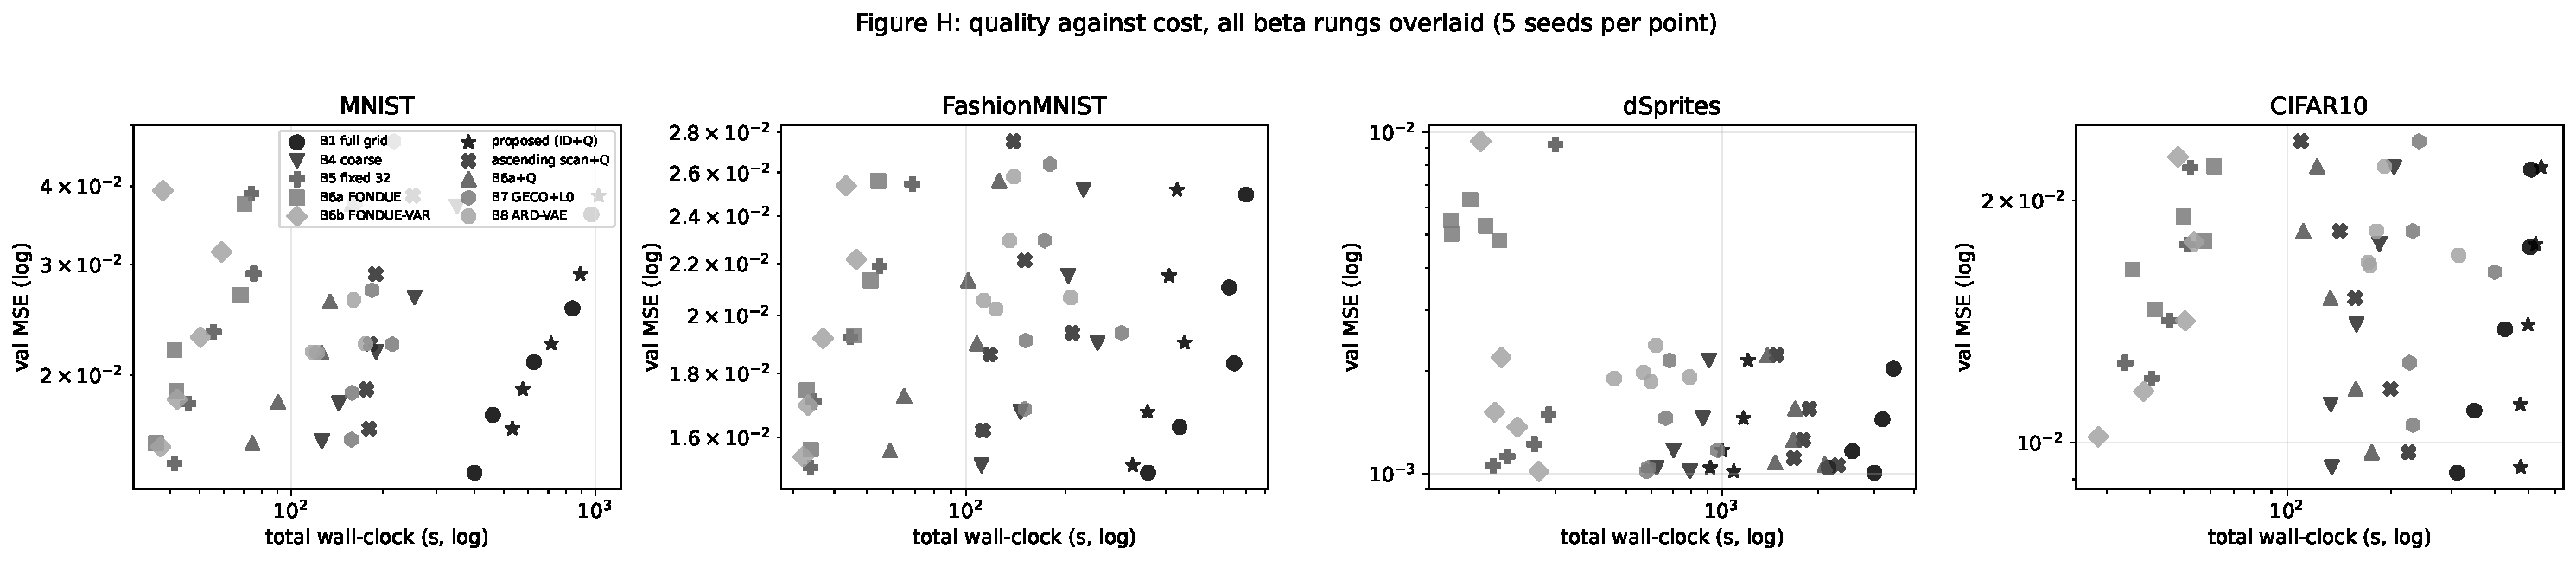
\includegraphics[width=\textwidth]{results/figures/MAKE49_FigH_quality_cost_beta.pdf}
\caption{Reconstruction error against total cost, with all five
regularisation settings overlaid. Five seeds per point; both axes
logarithmic.}
\label{fig:quality_cost}
\end{figure}

\subsection{Sensitivity of the Intrinsic-Dimension Estimate}\label{sec:res_id}

The quantity the guided procedure depends on is not a property of the data
alone. Estimating it in the input space, in a PCA-preprocessed space and
through trained reference autoencoders gives values that differ by a
factor of between about 1.7 and 3.7 on the same dataset
(Figure~\ref{fig:id_dependence}). Because the candidate window is placed
at twice the estimate, the window moves by the same factor.

The agreement between two standard estimators also depends on the size of
the estimation sample. With a thousand points all four datasets pass the
agreement criterion we fixed in advance; with ten thousand points only one
does. The decision to apply or to decline the procedure therefore depends
on a quantity that is free to choose. We fixed the sample size before
seeing any result, and we report the dependence rather than selecting the
value that would have let the procedure proceed.

\begin{figure}[H]
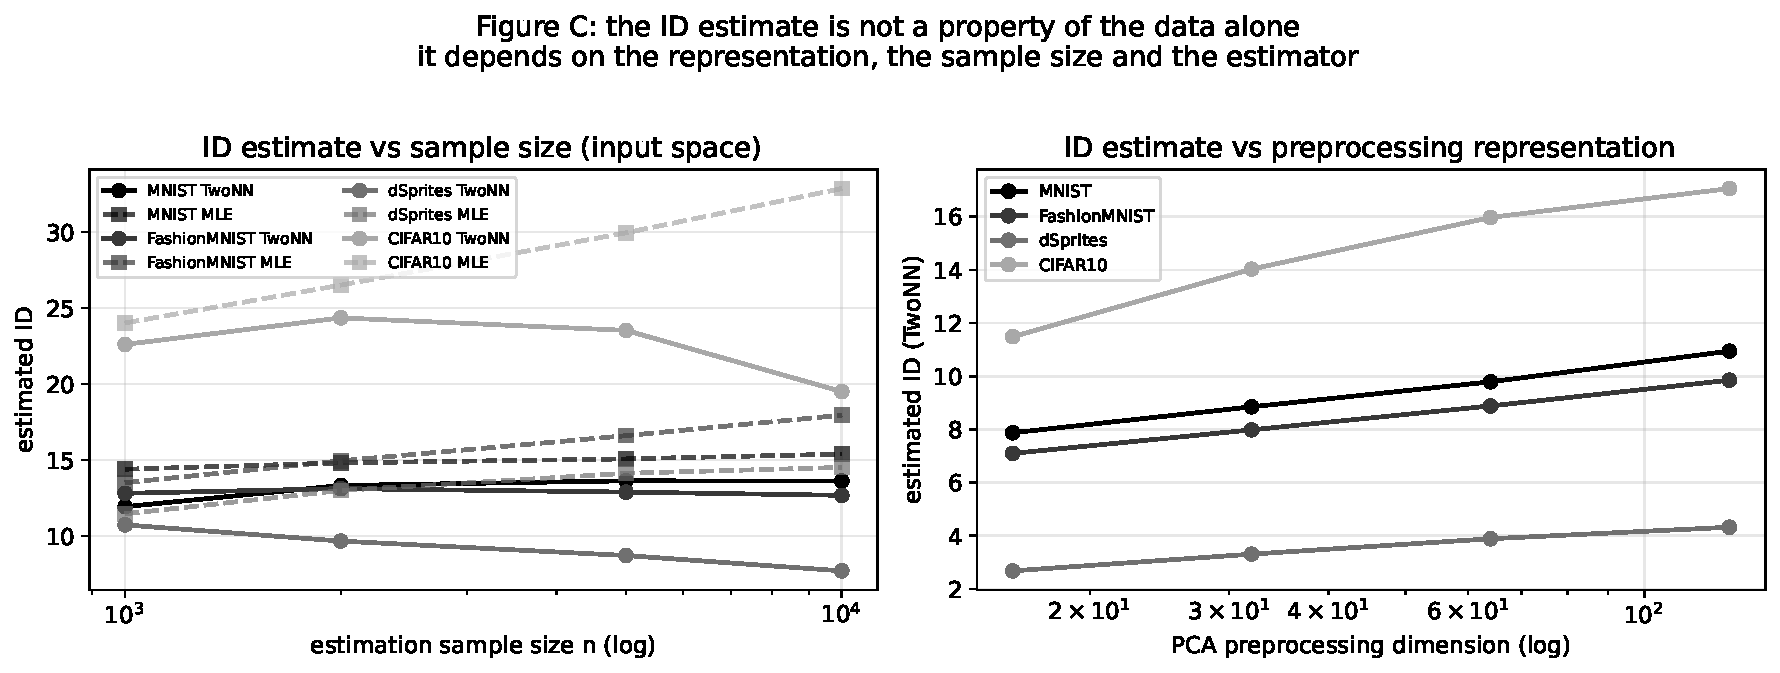
\includegraphics[width=\textwidth]{results/figures/MAKE49_FigC_id_dependence.pdf}
\caption{The intrinsic-dimension estimate as a function of the estimation
sample size (left) and of the preprocessing representation (right).}
\label{fig:id_dependence}
\end{figure}

On dSprites the estimate is 7.70 in the input space, between 2.68 and 4.32
in principal-component spaces of increasing rank, and between 2.08 and
4.56 through trained reference autoencoders of three capacities: a range
of 3.7 to one on a single dataset. On MNIST the corresponding range is 1.7
to one. The relative disagreement between the two estimators rises from
0.068 at a thousand points to 0.885 at ten thousand on dSprites, and from
0.063 to 0.686 on CIFAR-10.

\subsection{Threshold Governance and Its Ordering}\label{sec:res_threshold}

Varying the regularisation weight over five settings moves the dimension
that each method selects. Table~\ref{tab:threshold_span} reports the span
of the selected dimension across that ladder, and
Figure~\ref{fig:beta_dependence} plots it. The spans differ by two orders
of magnitude between methods, and the ordering is consistent across
datasets.

One method is flat. The automatic-relevance variant returns an identical
value at every rung on every dataset, because it has no free threshold to
vary: the relevance of each axis is read from a hierarchical prior fitted
to the data. Every other method we examined --- including plain grid
search under a reconstruction criterion --- moves substantially. This is
the clearest single result of the study: the question is not whether a
selection rule has a free parameter, but how strongly the answer depends
on it.

\begin{table}[H]
\caption{Span of the selected dimension across five regularisation
settings, by method and dataset. Smaller is less governed by the free
parameter; five seeds per setting.}
\label{tab:threshold_span}
\begin{tabularx}{\textwidth}{lCCCCC}
\toprule
\textbf{Method} & \textbf{MNIST} & \textbf{Fashion} & \textbf{dSprites}
& \textbf{CIFAR-10} & \textbf{Mean} \\
\midrule
Fixed dimension          & 0.0  & 0.0  & 0.0   & 0.0   & \textbf{0.0} \\
ARD-VAE                  & 0.0  & 0.0  & 0.0   & 0.0   & \textbf{0.0} \\
FONDUE                   & 3.8  & 0.8  & 0.8   & 8.8   & 3.5 \\
GECO + $L_0$             & 8.8  & 2.0  & 0.0   & 34.2  & 11.2 \\
Ascending scan + target  & 6.0  & 3.6  & 15.2  & 52.8  & 19.4 \\
FONDUE + quality target  & 3.6  & 1.6  & 28.0  & 44.8  & 19.5 \\
Grid search              & 14.8 & 20.8 & 40.0  & 91.2  & 41.7 \\
ID-guided + target       & 6.0  & 37.2 & 0.0   & 214.4 & 64.4 \\
Coarse search            & 33.6 & 37.2 & 0.0   & 214.4 & 71.3 \\
FONDUE-VAR               & 50.6 & 63.0 & 106.2 & 68.8  & \textbf{72.2} \\
\bottomrule
\end{tabularx}
\end{table}

\begin{figure}[H]
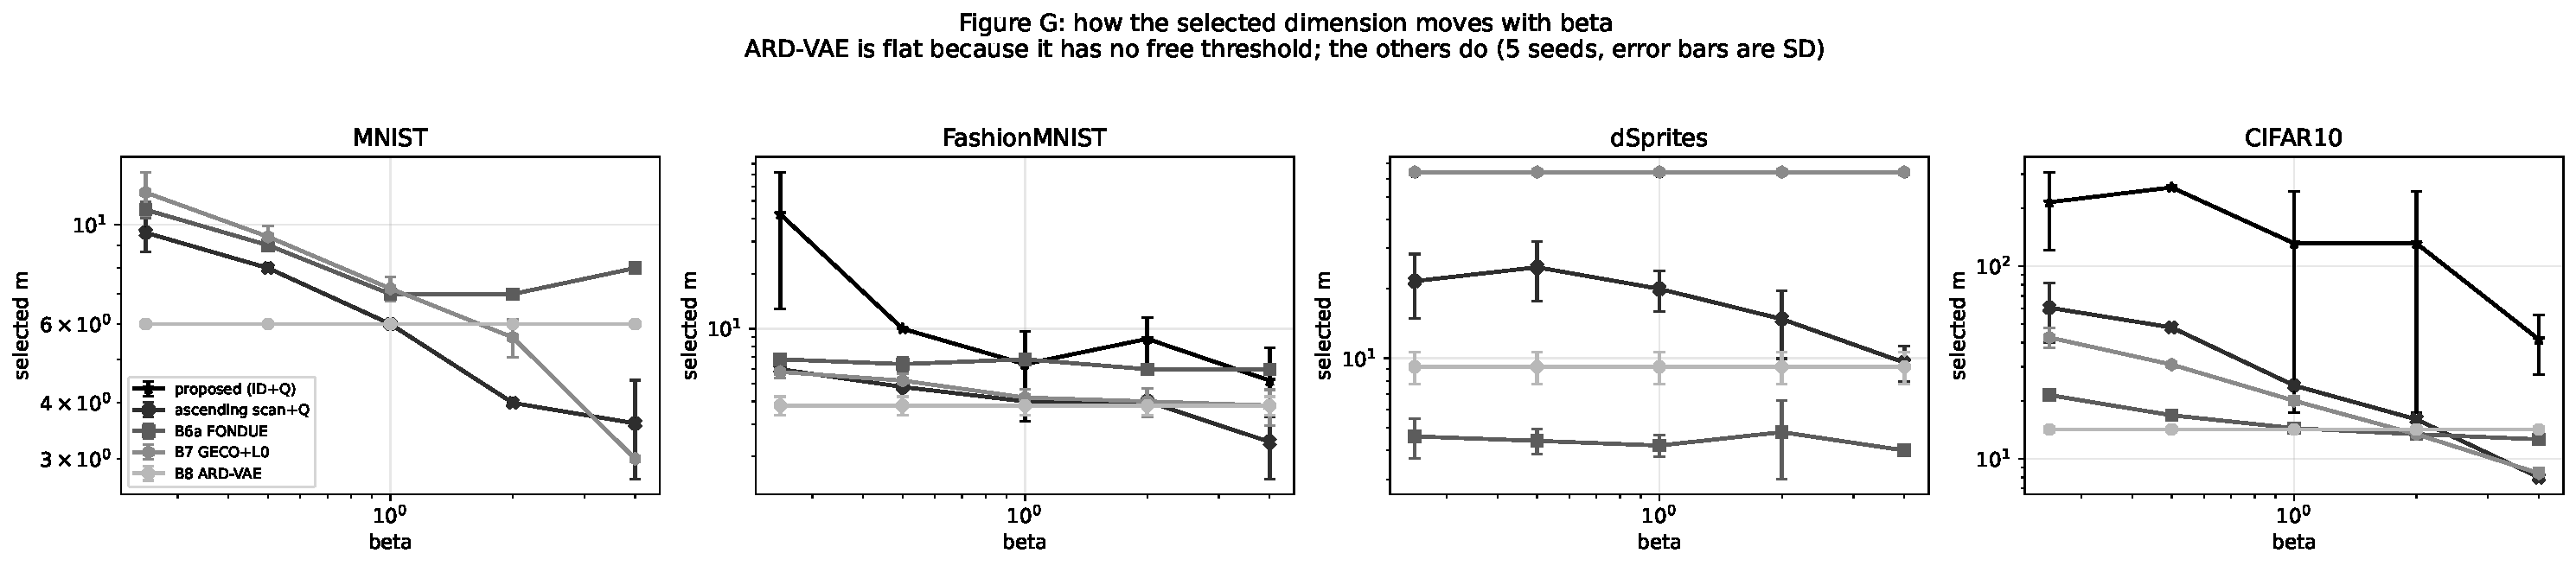
\includegraphics[width=\textwidth]{results/figures/MAKE49_FigG_beta_dependence.pdf}
\caption{Selected dimension against the regularisation weight, five seeds,
error bars are standard deviations. The automatic-relevance method is flat
on every dataset.}
\label{fig:beta_dependence}
\end{figure}

The spans differ by more than two orders of magnitude, from zero to 72.2
on average. Grid search under a reconstruction criterion, the least
elaborate rule in the comparison, has a mean span of 41.7: the premise
that fixing the regularisation weight fixes an optimal dimension does not
hold even there. The guided procedure sits at 64.4, inflated by CIFAR-10,
where it inherits the instability of the search it falls back to.

\subsection{Stability of the Activity Readout}\label{sec:res_au}

We compared two readouts computed from the same checkpoints: the number of
latent coordinates whose posterior means retain variance, and the
variable-type classification used by a published algorithm. Both are
unstable early in training and both stabilise by the end; by the final
checkpoint they agree closely, so the claim that one is more stable than
the other is not supported. At the earliest checkpoints the ordering is in
fact reversed on one condition.

The activity readout is governed by its own threshold. On natural images
the verdict reverses within the range of threshold values in common use:
at the small end no truncation is detected at any capacity, and at the
large end the count saturates well below capacity
(Figure~\ref{fig:delta_sensitivity}). Normalising the threshold by the
scale of the representation does not remove this dependence; it
reparameterises it.

We also asked whether the activity readout carries information that other
diagnostics do not, using a prediction task on held-out conditions defined
in advance. The pre-registered rule returned a positive verdict. A control
that adds the same number of random features to the same baseline produced
an improvement that cannot be distinguished from it. We therefore report
that the pre-registered test lacked the power to attribute the improvement
to the readout, and we do not claim incremental value.

\begin{figure}[H]
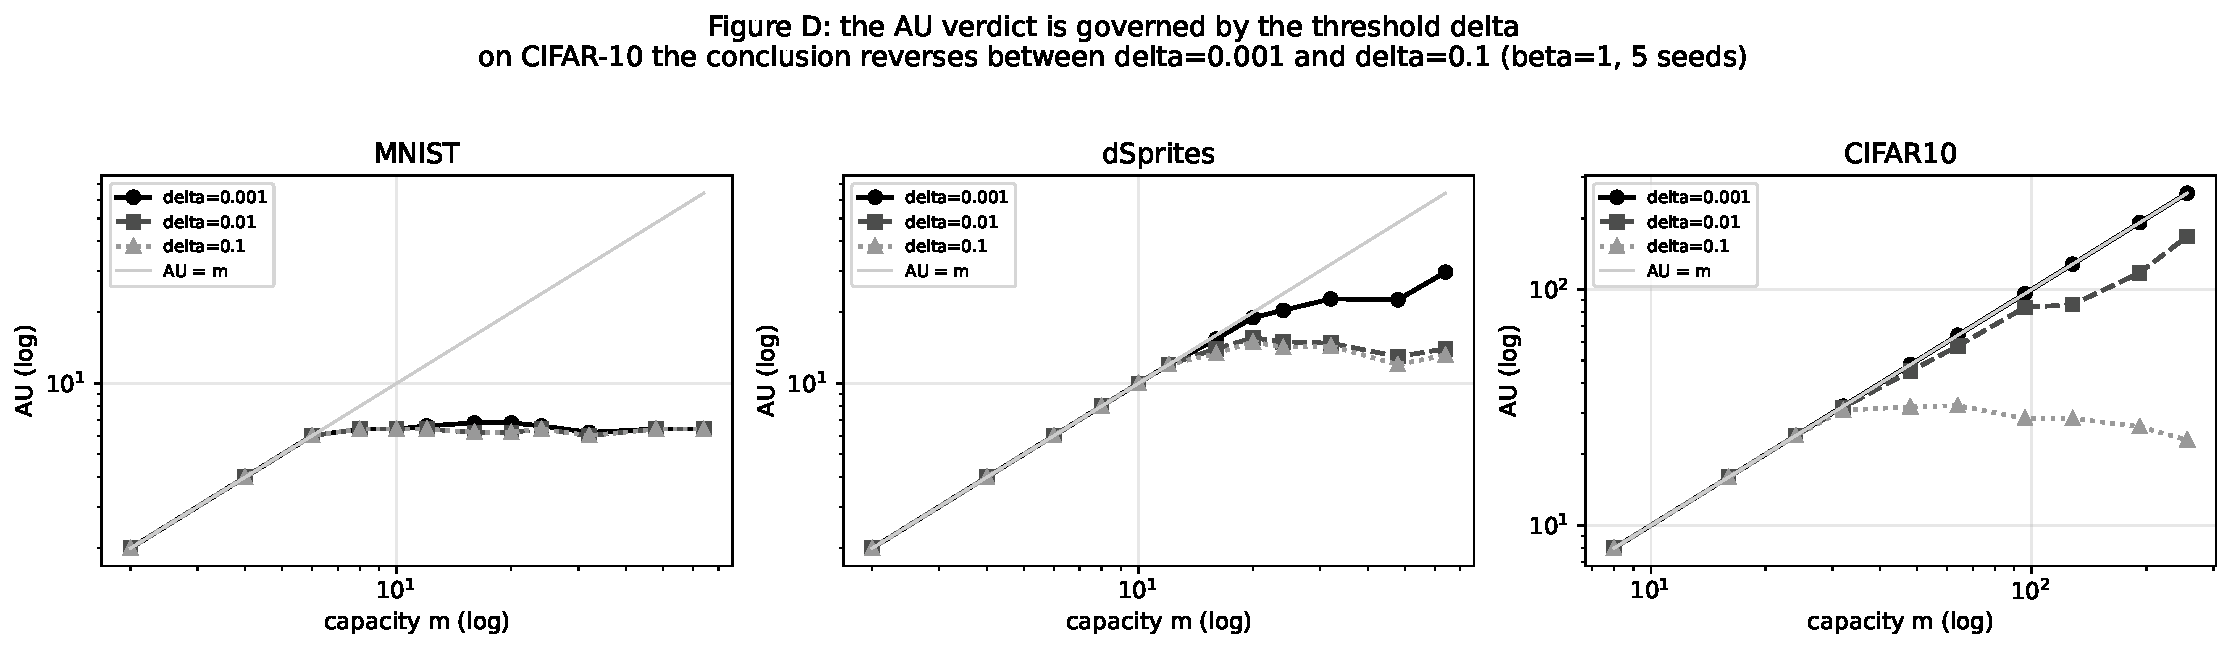
\includegraphics[width=\textwidth]{results/figures/MAKE49_FigD_delta_sensitivity.pdf}
\caption{Activity count against capacity for three settings of the
activity threshold. On CIFAR-10 the verdict reverses between the smallest
and largest setting.}
\label{fig:delta_sensitivity}
\end{figure}

On CIFAR-10 at the smallest threshold the count equals capacity in every
condition we ran, so no truncation is detected anywhere; at the largest it
saturates between 23 and 32 while capacity grows to 256. The
pre-registered prediction task gave a mean improvement in area under the
curve of $+0.108$ with a bootstrap interval of $[+0.059, +0.157]$,
which the registered rule reads as incremental value; a control adding
three random features to the same baseline gave $+0.098$ with interval
$[-0.025, +0.227]$, which the first interval does not exclude.

\subsection{Natural Images}\label{sec:res_natural}

On the two datasets other than MNIST for which the guided procedure was
run, the estimation step failed its own reliability checks on every seed
and the procedure declined to apply, falling back to the pre-declared
conventional search. The fallback was itself unstable on natural images.
The procedure succeeded only on the dataset used for development. We
therefore do not claim applicability to natural images.

On dSprites the three reference models gave estimates of 3.96, 3.91 and
2.10, a relative range of 0.474 against a criterion of 0.15, and the two
estimators disagreed by 1.816 against a criterion of 0.25. On CIFAR-10 the
checks failed likewise. In both cases the procedure returned the
unreliable state on all five seeds.

\subsection{Implementation Failure Modes}\label{sec:res_failures}

Three defects surfaced during this study, all of the same kind: a sum was
written as a mean, or the reverse, so that two terms of an objective were
weighted relative to each other by a factor of the order of the
dimensionality. None of them caused training to fail; each produced
plausible curves and would not have been visible in the reported numbers.

The first was in our own objective and affected every variational
experiment in the earlier version of this work. The second appeared in our
re-implementation of a pruning method and caused it to violate its own
reconstruction constraint while reporting a selected dimension. The third
is a degenerate output of a published algorithm under one of its declared
settings, which we reproduce faithfully and report as such rather than as
an error of that work. We describe all three, with the checks that now
guard against them, because this class of defect is invisible in
aggregate results and is a realistic hazard for anyone re-implementing
these methods.

In the first case the divergence term was averaged over latent dimensions
as well as over the batch while the reconstruction term was summed over
input dimensions, so the effective weight was the nominal weight divided
by the capacity. The previously reported dependence of the activity count
on capacity is reproduced to within 1.7 units by re-reading it as a
function of that ratio. In the second, a reconstruction constraint was
evaluated as a per-pixel mean where its source defines it as a sum over
pixels, leaving it smaller by the input dimension than the term it was
meant to balance; the method then pruned from 64 dimensions to 1 while
violating the constraint it reports satisfying. In the third, the
variable-type algorithm under one of its two declared settings returns an
active count of zero on MNIST at the epoch budget its authors use, on all
five seeds.

\section{Discussion}\label{sec:discussion}

\subsection{What the Comparison Shows}\label{sec:disc_main}

The question we set out to answer was which of the available signals
supports the choice of a latent dimension. On the evidence collected here,
the intrinsic-dimension estimate does not. It is expensive to obtain,
it depends on the representation in which it is computed, and a search
that ignores it entirely reaches the same answer sooner. The activity
readout does not either: it agrees with the alternative readout once
training has finished, its verdict on natural images reverses with its own
threshold, and in a prediction task designed in advance it was not
distinguishable from random features of the same number.

What remains is less a method than a measurement. Almost every rule we
examined is governed by a free parameter, and the dimension it selects
moves severalfold as that parameter varies. The spans in
Table~\ref{tab:threshold_span} differ by two orders of magnitude between
methods, and the ordering reproduces across datasets. That ordering is the
most transferable thing we found.

\subsection{Relation to Existing Work}\label{sec:disc_related}

Two points of overlap deserve to be stated plainly rather than discovered
by a reader. First, the appendix of the intrinsic-dimension algorithm we
compare against already proposes selecting the dimension from the
variable types of a briefly trained model, which is the same idea as the
activity-based verification we set out to study; its authors set it aside
for reasons our measurements reproduce. Second, the pruning method we
added during revision already selects the smallest capacity that satisfies
an explicit reconstruction constraint. The quality criterion we use
throughout this paper is the same construction. We therefore do not claim
it as a contribution, and we report the correspondence quantitatively: the
dimension that method selects tracks the constraint we set for it across
the whole ladder.

\subsection{What Would Change the Conclusion}\label{sec:disc_limits}

These are observations under one architecture family per dataset, one
candidate grid, five seeds and five regularisation settings. They do not
establish that intrinsic dimension is uninformative in general; they
establish that under these conditions it bought nothing that a cheaper
search did not. A different quality target, a capacity range where
reconstruction still improves steeply, or a dataset whose estimate is
stable across representations could each change the balance. The
measurement we would trust to transfer is the sensitivity ordering, not
the individual selected dimensions.

Two comparisons remain absent. Our re-implementation of the
intrinsic-dimension algorithm does not reproduce its published value on
the one dataset where a published value exists, so that value stays in a
reference column and the gap stands. The pruning method is implemented
with a different gradient estimator than its authors used, and the
relevance method with a Gaussian approximation in place of the
marginalised prior; both deviations are stated where the methods are
defined.

\subsection{Synthetic Versus Real Data}\label{sec:disc_synth}

On standardised synthetic manifolds with a known embedding dimension the
activity readout behaves as the topological argument would suggest: it
saturates at the embedding dimension, and zeroing the coordinates it
excludes changes reconstruction by less than a fifth of a percent. An
earlier version of this work reported the opposite on one manifold; that
observation was an artefact of leaving the coordinates unstandardised,
where one axis carried two parts in a thousand of the variance and could
be ignored at almost no cost. The contrast between the synthetic case,
where the readout works, and the image datasets, where its verdict is set
by its threshold, is itself the finding we would carry forward.

\section{Conclusions}\label{sec:conclusion}

We compared the signals that have been proposed for choosing the latent
dimension of a variational autoencoder, under a protocol fixed before the
experiments and across four datasets, five seeds and five regularisation
settings. Guidance by an intrinsic-dimension estimate conferred no
measurable advantage over an ascending search under the same quality
criterion, and declined to apply on the image datasets it was not
developed on. The activity-based readout was not more stable than the
alternative it was meant to improve on, and carried no information beyond
a matched set of random features. The quality criterion that did transfer
is not ours; it coincides with the constraint used by an existing pruning
method.

What we can offer is a measurement rather than a method: a reproducible
ordering of how strongly each rule's answer depends on its free parameter,
with one method at zero and another spanning more than a hundred
dimensions on the same data. We also record three implementation defects
of a single kind, invisible in aggregate results, that anyone
re-implementing these methods is likely to meet.

\end{document}
